\documentclass[12pt]{article}
\usepackage{fontspec}
\usepackage{anyfontsize}
\usepackage[letterpaper, margin=1in]{geometry}

\usepackage{graphicx}
\usepackage{tabularx}
\usepackage{subcaption}
\usepackage{parskip}
\usepackage[nottoc,numbib]{tocbibind}
\usepackage{hyperref}
\usepackage{biblatex}
\hypersetup{hidelinks = true}

\bibliography{references}

\newfontfamily{\atnight}{At-Night}[Path = font/, Extension = .ttf]

\begin{document}

\begin{titlepage}
    \begin{center}
        \vspace*{1cm}
 
        {\fontsize{60}{75}\atnight Skrach}
 
        \vspace{0.5cm}
        \Large
        An FPGA MIDI Synthesizer
 
        \vspace{3cm}
 
        \textbf{by\\Daria Solovey}
 
        \vfill
        
        \Large
        A Technical Report Submitted to the Faculty of the\\
        Department of Computer Science and Engineering\\
        University of [REDACTED]\\
        
        \vspace{1cm}
        Submitted in partial fulfillment for the requirements of\\
        CE446--Advanced Embedded Systems\\
        May 3rd, 2020
 
    \end{center}
\end{titlepage}

\tableofcontents

\newpage

\section{Introduction/Foreword}
CE446 is an advanced embedded systems class aimed at teaching students advanced techniques for designing embedded systems that accomplishes specific goals or solving problems. The class centers around the use of FPGAs with hardware design in VHDL, designing solutions in hardware rather than using higher level programming in micro controllers. As an extension of the FPGA, softcores are also used such as the MicroBlaze microprocessor. The final assignment of the class was to explore a topic and engineer a solution to a student's topic.

I chose to explore digital synthesis of sound and its application in music: creating oscillators and interfacing with external controllers that utilize the MIDI protocol. Personally, I've always been curious as to what goes into creating a proper synth, having worked with many virtual synthesizers over the years. In the context of the report, I am an engineer who works at Quantum Fidelity (a company I may actually register or even open).

\section{Design Goals}

These are the initial design goals developed at the start of the project. As the project progressed, some initial ideas changed and were even thrown out all together due to time constrains or difficulty.

\subsection{Need Statement}

Quantum Fidelity, a tech startup, is looking to develop a synthesizer module not dissimilar to classic systems such as the Moog, Yamaha DX7, and Korg synths. In this case, instead of a built in keyboard, as many classical synths used, the system will be controlled via MIDI protocol, allowing for agnostic control over the synth.

\subsection{Marketing Requirements}

The basic requirements of the Skrach Synth are as follows:

\begin{itemize}
    \item Generate signals such as a sine, triangle, square, and saw, outputting samples as audio.
    \item Interface with controllers over MIDI protocol using a standard 5 pin MIDI connector, allowing for receiving of control signals.
    \item Modulate the pitch of the signals generated by the synth using MIDI note events generated by a controller.
    \item Print debug info as well as allow for control using serial console over UART.
\end{itemize}

\noindent Advanced requirements are as follows:

\begin{itemize}
    \item Interface with control elements such as nobs, faders, and pads on a MIDI device to control the system.
    \item Add filters, effects, and envelopes to the generated signals to allow for even more sound characteristics.
    \item Modify the characteristic of the signal via frequency modulation like the mentioned commercial synthesizers.
    \item Use audio input as a signal to modulate, similar to vocoder systems, also implemented in some commercial synthesizers.
\end{itemize}


\noindent Future ideas which are not requirements:

\begin{itemize}
    \item Video output showing an interface that shows the state of Skrach, especially the shape of the signal being output through the system and levels and settings of the synth.
    \item MIDI Clock sync so that you can use multiple MIDI devices on the same synth, or synchronize sequencer functionality with controllers.
\end{itemize}

\subsection{Level-0 Design}

\begin{figure}[htb]
    \centering
    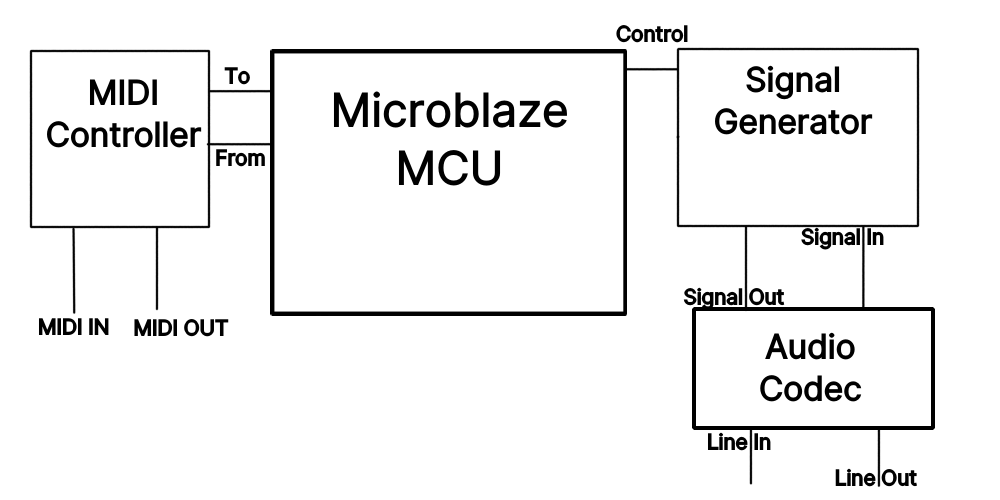
\includegraphics{img/level_0_diagram.png}
    \caption{Level 0 diagram showing I/O and initial system overview}
    \label{fig:level_0_figure}
\end{figure}

\begin{table}[htb]
    \centering
    \begin{tabularx}{\linewidth}{r|l}
        Module  & Skrach Synth \\\hline
        
        Inputs  & Serial control over UART (USB)\\
                & 5 pin MIDI input for control input from MIDI devices\\
                & \emph{Advanced}: Audio input via Mic or Line In\\\hline
                
        Outputs & Audio of the signal being generated on Line Out\\
                & Debug information on serial console over UART\\
                & \emph{Future}: Video showing state of the system and signal being generated\\
                & \emph{Future}: MIDI Out for clock sync and other related settings/functions\\\hline
        Behavior& 1. Startup generates basic sine wave and output to audio.\\
                & 2. Use switches to change type of signal (sine, square, etc)\\
                & 3. MIDI signals from MIDI peripheral maps to certain functionality in\\
                & \ \ \ \ synth, namely keyboard keys to pitch of the signal\\
    \end{tabularx}
    \caption{Level-0 Functionality}
    \label{tab:level_0_table}
\end{table}

\newpage

\section{Detailed Design}

As more thought was put into the system and the concepts researched, an initial detailed design was created.

\subsection{Level-1 Description}

The keyboard depicted in the figure is the MIDI controller being used for testing of the system. As such, some functionality may be programmed to better suit the particular keyboard's implementation of the MIDI protocol.

The MIDI circuit is credited to MIDI.org, the organization which oversees the development of the protocol.

\begin{figure}[htb]
    \centering
    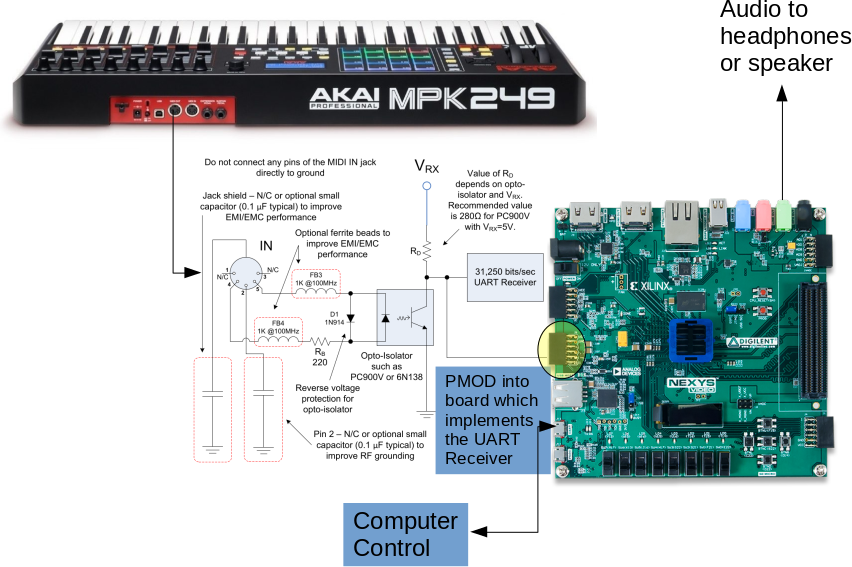
\includegraphics[width=0.75\textwidth]{img/level_1_diagram.png}
    \caption{Level 1 user interaction graphic}
    \label{fig:level_1_figure}
\end{figure}

\subsection{Datapath and Control}

Within the Skrach Core there are 12 operators which are instantiated and mixed together using as single mixer instance. The diagram is simplified in that respect.

\begin{figure}[htb]
    \centering
    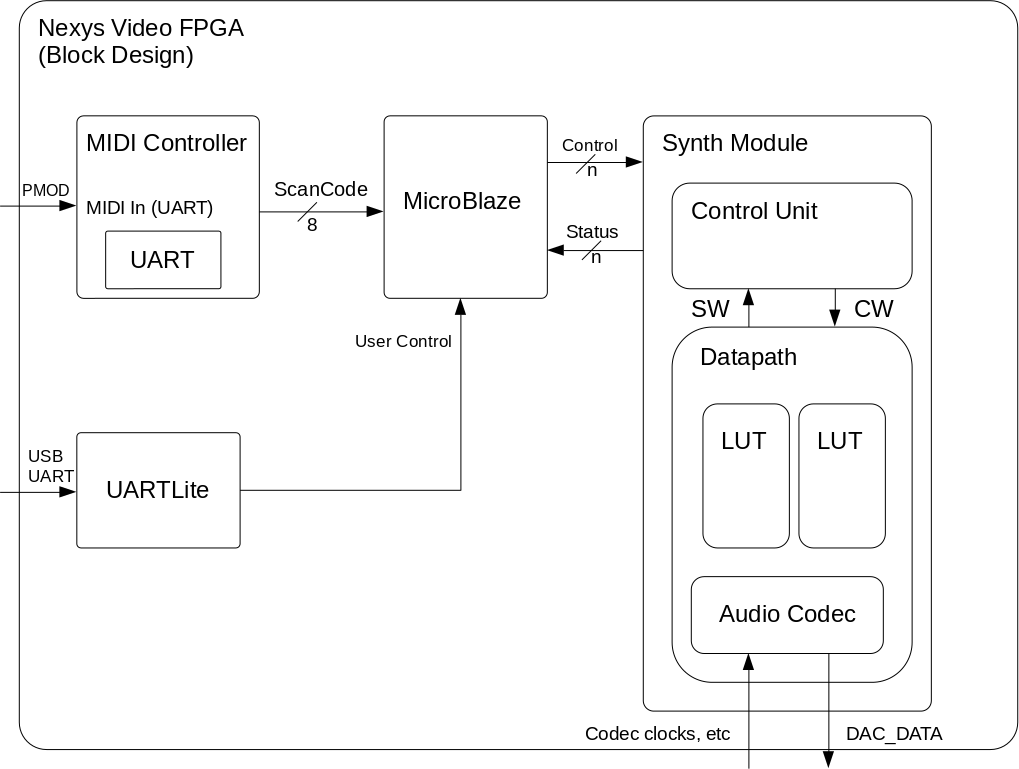
\includegraphics[width=\textwidth]{img/datapath_conrol.png}
    \caption{Skrach block diagram}
    \label{fig:block_diagram}
\end{figure}

The major control pieces are the UART control for user input, and also MIDI control which also works over UART. (control)

Both feed into the MicroBlaze which will then control the synth module (datapath), modifying frequency, amplitude, and sound shape for output.

\subsection{Calculations}

\subsubsection{Synth Module}

The synth module will implement look up tables with phase accumulation to be able to change frequency. This will involve a Q9.7 phase signal to do step changes in indexing. Interpolation may be implemented to help make the signal more accurate; however, at higher sample counts, it may not be all that necessary.

Once more research is done on how to perform FM Synthesis, that too will be implemented using low frequency oscillators to modulate the carrier signal (main output). This may involve the addition and multiplication of sample data.

A filter and envelope system will also be implemented that allows for control of the signal's output in amplitude. This will entail the multiplication of signals as well.

\subsubsection{MIDI Controller}

The MIDI controller doesn't have much for calculation other than decoding the UART signal as it comes it. The signal is an 8 bit scan code control signal signifying changes on the MIDI Device with a start and stop bit, meaning a total of 10 bits per control element.

A state machine will have to be devised to read this properly and accurately. Either that, or an already available UART controller such as the UART Lite modified to work with the MIDI protocol.

\subsubsection{MicroBlaze}

For control, once scan codes are decoded from MIDI, the phase should change depending on what key was pressed. A popper frequency needs to be calculated and output as control to the synth module in the form of a Q9.7 phase value.

This can be summed up in the following equation:

\begin{equation} \label{eq:phase}
    \Phi = \frac{Nf}{F_s} 
\end{equation}

Where $\Phi$ is the phase, $N$ is the number of samples per period, $f$ is the desired frequency, and $F_s$ is the audio sampling frequency.

When reading from the synth the phase and converting to frequency, the equation can be rearranged such that $f$ is on the left hand side, and $\Phi$ is on the right.

Another equation to consider is what frequency corresponds to what keyboard key as dictated by a standard 88 key piano. A suitable equation was found online in the context of the MIDI protocol \cite{wolfe}:

\begin{equation} \label{eq:midi_freq}
    f = 2^{\frac{m-69}{12}}(440)
\end{equation}

Where $f$ is the desired frequency and $m$ is the midi key assuming the note $A_4$ is at 440Hz.

\subsection{Technical Requirements}

Similar to the marking requirements, theses are the basic requirements that need to be met to be able to achieve the design goals:

\begin{itemize}
    \item Ability to receive and properly decode MIDI signal allowing 88 keys of input as well as some basic control elements such as faders and knobs.
    \item With MIDI input, allow for basic polyphony of input, meaning multiple inputs can be handled at once, but not necessarily in sound (be able to hold a note down while changing the volume of sound).
    \item Ability to print the status of the system over UART to a console as well as allow user input to control aspects of the synth module.
    \item Output a 16bit 48kHz audio signal so that the system is a fairly high fidelity in terms of audio output.
\end{itemize}

\subsection{Bill of Materials}

There are 3 major pieces to this project:

\begin{itemize}
    \item Nexys Video FPGA
    \item MIDI Input Circuit (optocoupler, diode, MIDI connectors)
    \item MIDI Controller such as a keyboard (AKAI MPK249)
\end{itemize}


\section{Implementation}

This section covers the process of implementing the technical requirements outlined in the previous section.

\subsection{Milestone I}

By the deadline, only the circuit had been built and tested through a logic analyzer that did decode. After spending some more time the following day, MIDI decode of status, pitch, and velocity through the MicroBlaze system was achieved. More work needed to be done to be able to implement more controller functionality so that things like faders and knobs can also be properly used. A data structure also had to be implemented to be able to easily and properly pass around MIDI events within the processor.

\subsubsection{Unit Test Plan}

The MIDI circuit first needed to be build and then made sure operational. For this, a breadboard and alligator clips was used to connect the circuit to the MIDI interface on the MIDI controller. The circuit was then connected to a logic analyzer and modified until proper communication was achieved. Once the circuit was working, components were cut in length to reduce possibility of shorts and wires were soldered to the MIDI connector to maintain good connection. Had there been access to a through-hole prototyping PCB, all the components would have been soldered together to prevent shorts and maintain proper contacts in the circuit. Figures \ref{fig:midi_in_schematic}, \ref{fig:logic_key_down}, and \ref{fig:logic_key_up} illustrate the final circuit used, as well as logic analyzer results.

\begin{figure}[!htb]
    \centering
    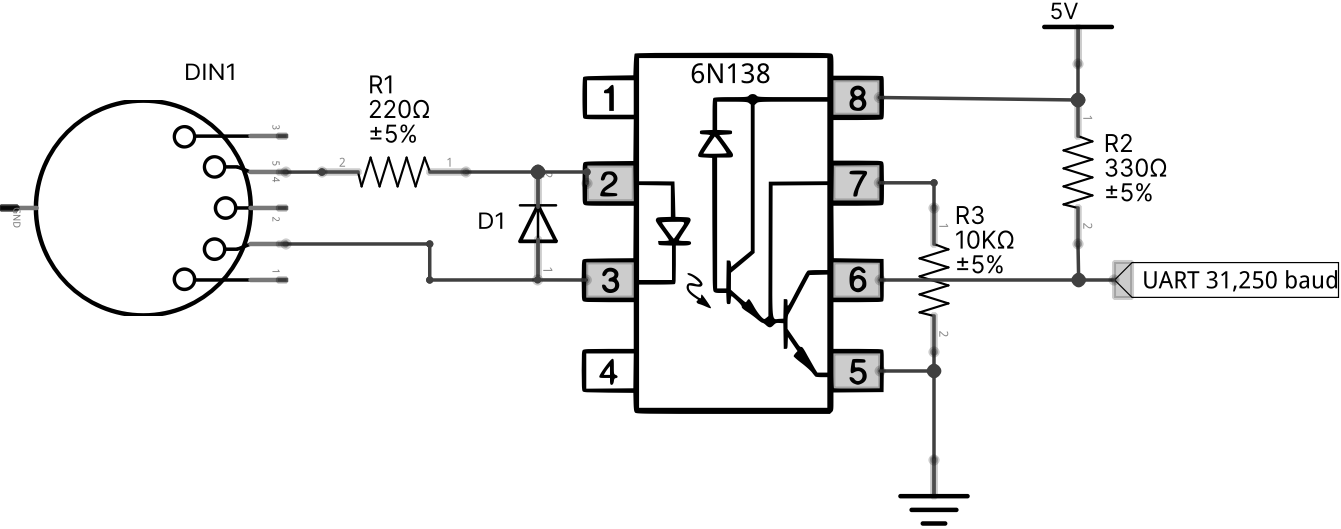
\includegraphics[width=\textwidth]{img/midi_in_schematic.png}
    \caption{MIDI in circuit schematic}
    \label{fig:midi_in_schematic}
\end{figure}

\begin{figure}[!htb]
    \centering
    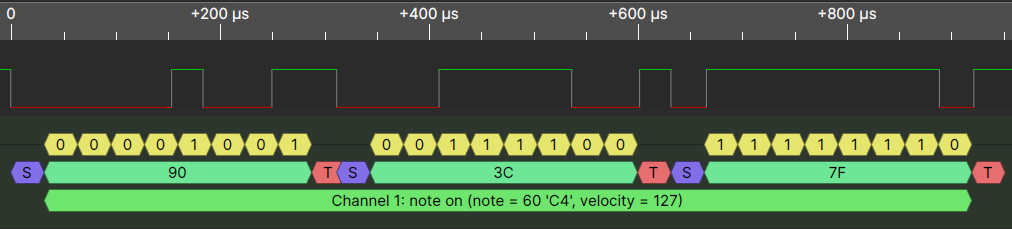
\includegraphics[width=\textwidth]{img/logic_analyzer_key_down.png}
    \caption{Logic analyzer MIDI key down read}
    \label{fig:logic_key_down}
\end{figure}

\begin{figure}[!htb]
    \centering
    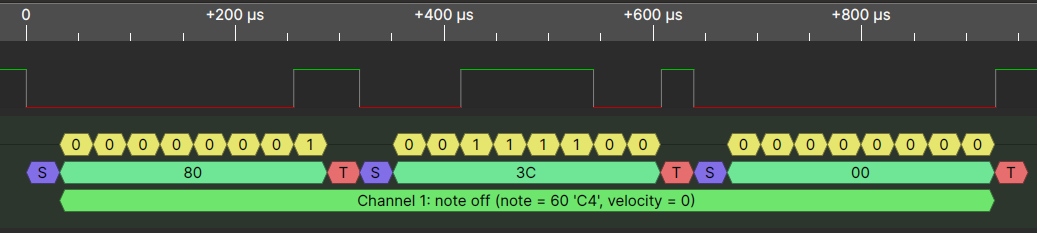
\includegraphics[width=\textwidth]{img/logic_analyzer_key_up.png}
    \caption{Logic analyzer MIDI key up read}
    \label{fig:logic_key_up}
\end{figure}

After the MIDI circuit was deemed complete, a previous project encompassing a MicroBlaze implementation was used as a starting point and copied. The UARTLite IP Core was copied into the local IP repo and edited to support the required baud rate of 31250. This new UARTLite was then added and had its RX pin connected to a PMOD port on the FPGA. As MIDI involves a 3 byte sequence, 3 calls to the UART read function were called and the data was printed to console. Once reading of data was tested, functions were written to start to decode the scan codes and map them to user friendly names. These were input into enumerated types and ultimately, a structure of 3 int variables was created to handle the data as a packet involving a control word, pitch, and velocity, as dictated by the MIDI protocol. By the second day after the deadline, decode of essential MIDI messages was fully implemented and data printed nicely to console. This is visible in figure \ref{fig:midi_decode}

\begin{figure}[htb]
    \centering
    \begin{subfigure}{.49\textwidth}
        \centering
        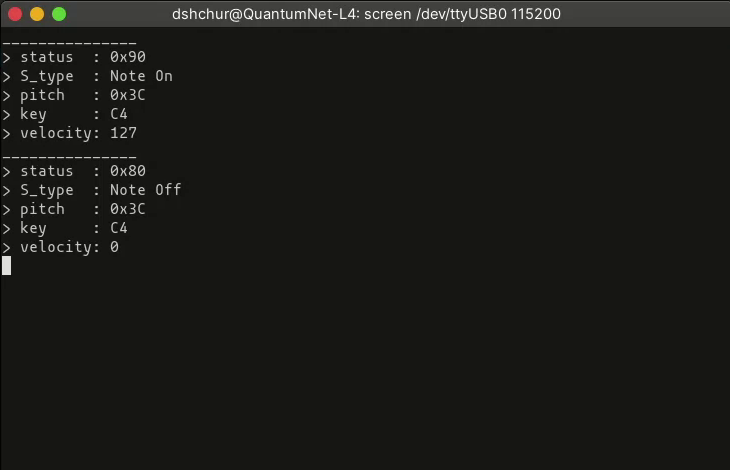
\includegraphics[width=\linewidth]{img/midi_decode_note.png}
        \caption{Note Event}
        \label{fig:decode_note}
    \end{subfigure}
    \begin{subfigure}{.49\textwidth}
        \centering
        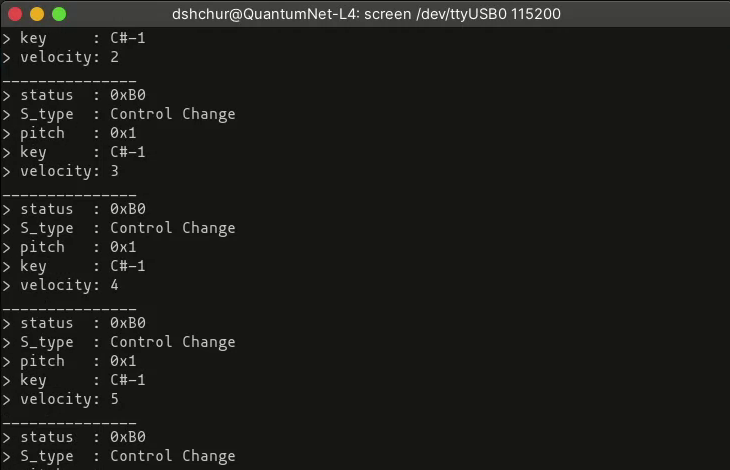
\includegraphics[width=\linewidth]{img/midi_decode_control.png}
        \caption{Control Event}
        \label{fig:decode_control}
    \end{subfigure}
    \begin{subfigure}{.5\textwidth}
        \centering
        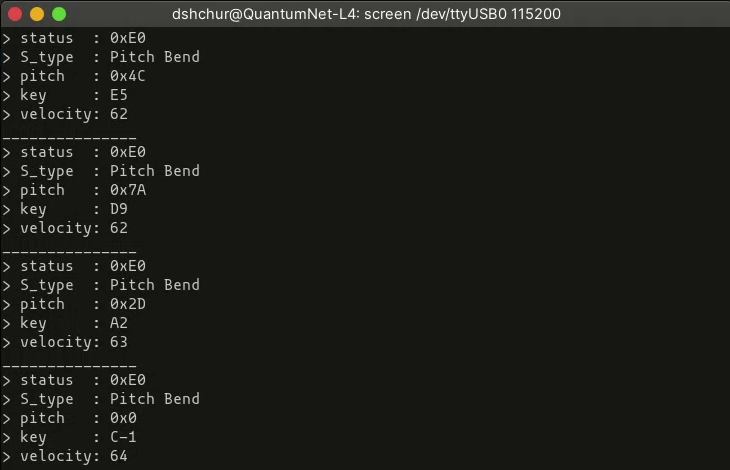
\includegraphics[width=\linewidth]{img/midi_decode_pitch.png}
        \caption{Pitch Event}
        \label{fig:decode_pitch}
    \end{subfigure}
    \caption{Basic MIDI decode}
    \label{fig:midi_decode}
\end{figure}

\subsection{Milestone II}

The goal for this milestone was to reuse a previous signal generator design from previous assignments and retrofit it to be controlled by MIDI.

The previous assignment IP was modified, removing hardware control since the system was begin controlled by the MicroBlaze. Control of the IP was implemented within the MicroBlaze, implementing equation \ref{eq:phase} for the required phase for the signal generator as well as equation \ref{eq:midi_freq} for MIDI. However, the inclusion of the IP block into the block design broke UART communication, this also includes the module related to MIDI reading. Because of the circumstances, the implementation was not able to be tested.

\subsection{Final Implementation}

In summary, the final implementation was able to do the following:

\begin{itemize}
    \item Read a MIDI device and decode MIDI messages.
    \item Generate a signal of type sine, triangle, saw, and square, implementing an oscillator.
    \item Modulate that signal using an amplitude envelope implementing attack, decay, sustain, and release (ADSR).
    \item Mix multiple signals together allowing for multiple oscillators to be combined, essentially allowing for polyphony.
    \item Modulate overall signal amplitude (volume).
    \item Output that signal using the audio codec at 48kHz sampling rate and 16bit width samples.
    \item Change pitch of oscillator using the data given by a MIDI note event.
    \item Start and stop playback of an oscillator upon receiving note on/off events.
    \item Adjust the ADSR envelope using MIDI control.
    \item Switch signal type using MIDI control.
    \item Play up to 12 notes at a time.
\end{itemize}

Some advanced functionalities such as frequency modulation and filters were not achieved due to lack of time. One basic requirement was also not acheived due to the complexity of doing so, which is UART control. Since there are two UART controllers in the system, either the MIDI or USB could be polled, but not both. This would have required setting one up on an intterrupt system, and that was not able to be achieved properly.

The modules are explained in the following sub-sections:

\subsubsection{Operator}

An operator consists of an oscillator and ADSR where the oscillator feeds directly into the ADSR, and ADSR feeds out.

\paragraph{Oscillator}

The oscillator is a signal generator, not dissimilar to that which had been created for a previous assignment, that can generate a sine, triangle, saw, and square wave. The frequency that is generated is determined by a phase accumulator which changes the step size of the system. The phase value is implemented as a Q9.7 fixed point value which allows for fine grained control of the frequency with a minimum of about .35Hz and maximum of 24kHz. The sine wave is stored as 16-bit samples in a 2048 address 36kb block of BRAM. A counter steps through the BRAM according to the phase value. The saw wave is simply the output of the address counter. The square wave is a mux which outputs the minimum value of a signed 16 bit signal while the counter is below 1024, and then maximum when the counter is above. Similar to the saw wave, the triangle is generated by doubling the address counter and negating it after 1024. No linear interpolation is performed.

The signals were confirmed using an oscilloscope as can be seen in figure \ref{fig:oscillator}.

\begin{figure}[htb]
    \centering
    \begin{subfigure}{.49\textwidth}
        \centering
        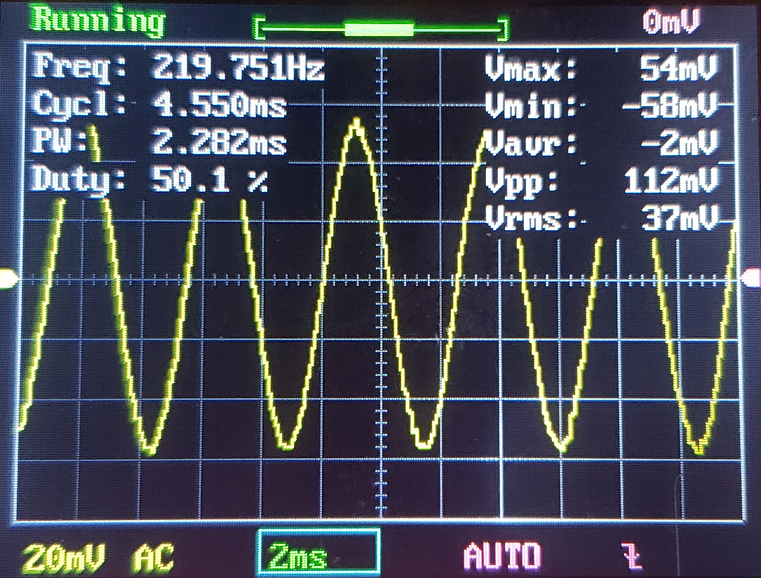
\includegraphics[width=0.75\linewidth]{img/sine.png}
        \caption{Sine}
        \label{fig:sine}
    \end{subfigure}
    \begin{subfigure}{.49\textwidth}
        \centering
        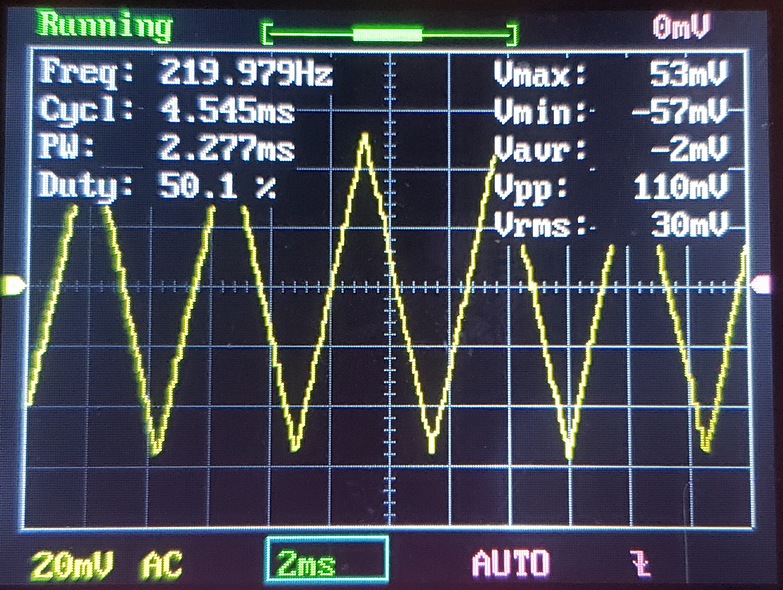
\includegraphics[width=0.75\linewidth]{img/triangle.png}
        \caption{Triangle}
        \label{fig:triangle}
    \end{subfigure}
    \begin{subfigure}{.49\textwidth}
        \centering
        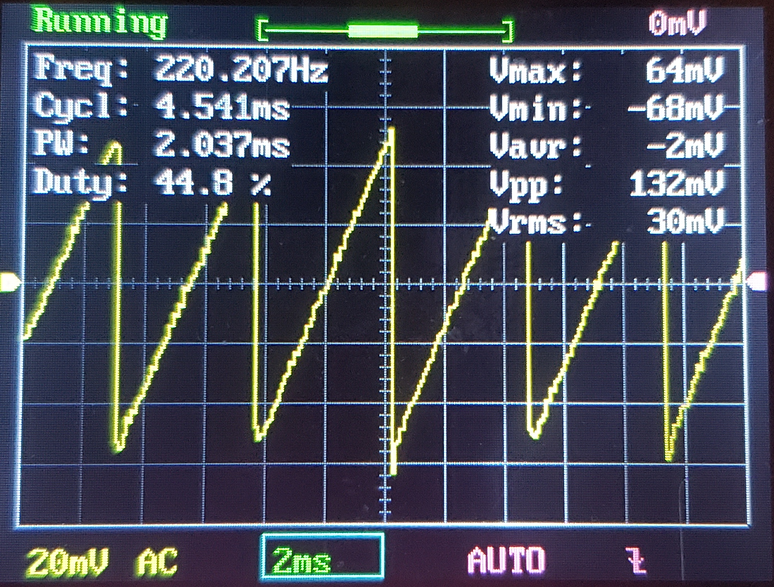
\includegraphics[width=0.75\linewidth]{img/saw.png}
        \caption{Saw}
        \label{fig:saw}
    \end{subfigure}
    \begin{subfigure}{.49\textwidth}
        \centering
        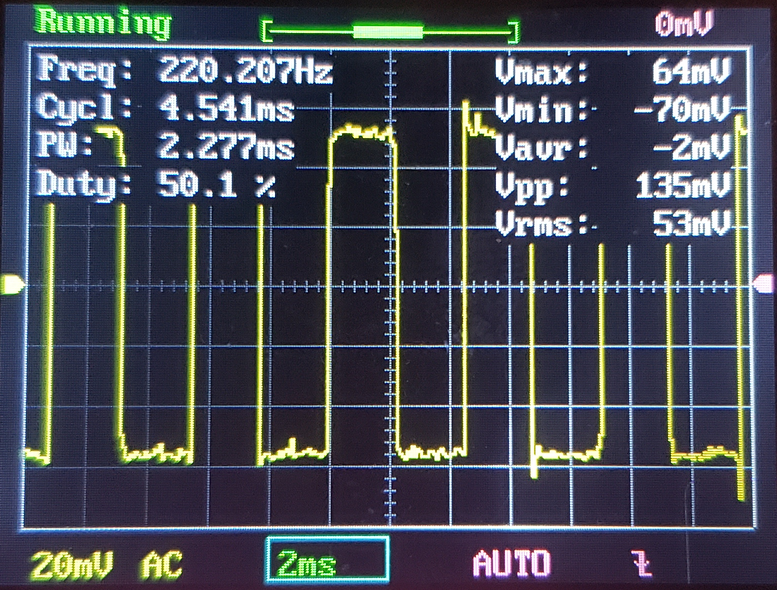
\includegraphics[width=0.75\linewidth]{img/square.png}
        \caption{Square}
        \label{fig:square}
    \end{subfigure}
    \caption{Oscillator outputs at 220Hz}
    \label{fig:oscillator}
\end{figure}

\paragraph{Amplitude Envelope (ADSR)}

An amplitude envelope is historically 4 variable system that dictates the amplitude of something over time. Within the synth, it was implemented with attack, decay, sustain, and release (ADSR). Attack, decay, and sustain are timing values, while sustain is an amplitude value. Attack corresponds to the amount of time it takes for the signal to read full amplitude, decay to the amount of time it takes for the signal to go from full amplitude to the level dictated by sustain, and release the amount of time it takes to bring the amplitude to zero from the level dictated by sustain \cite{wiki_adsr}.

It was implemented as a state machine where, upon being enabled, it would start the attack and continue through to decay, and then sustain. It would stay in sustain until it was no longer enabled, at which it would go to release. If during release, it was enabled again, it would jump to attack. If during attack, decay, or sustain it was disabled, it would move to release.

Figures \ref{fig:adsr1} and \ref{fig:adsr2} show the amplitude of the signals corresponding to values set by the MIDI controller where attack is the left most fader, followed by decay, sustain, and release.

\begin{figure}[htb]
    \centering
    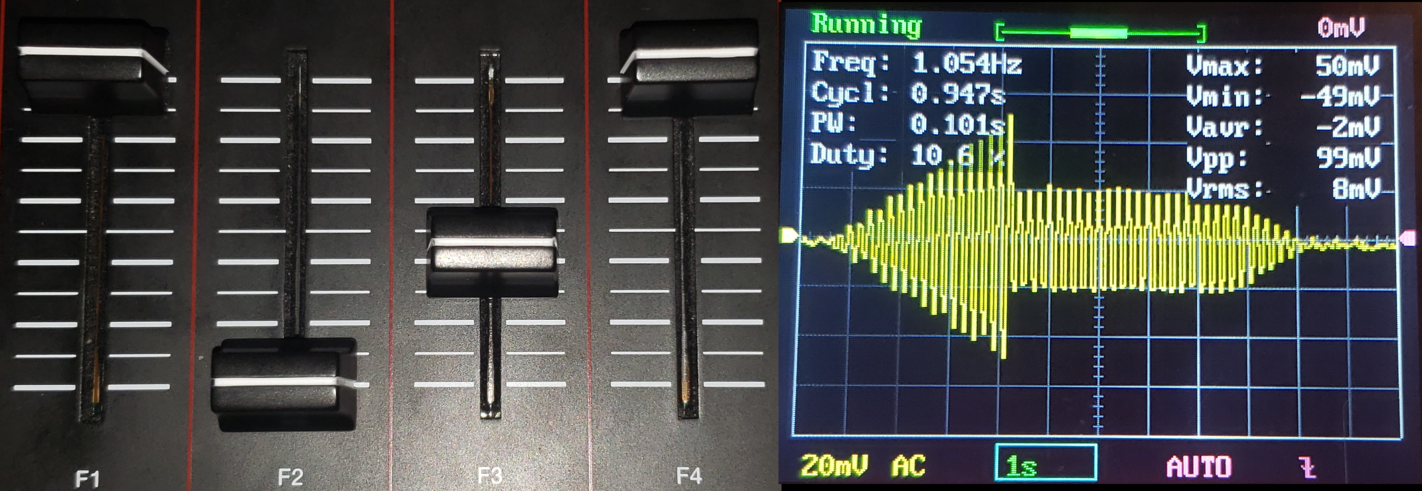
\includegraphics[width=\textwidth]{img/adsr1.png}
    \caption{ADSR 1}
    \label{fig:adsr1}
\end{figure}

\begin{figure}[htb]
    \centering
    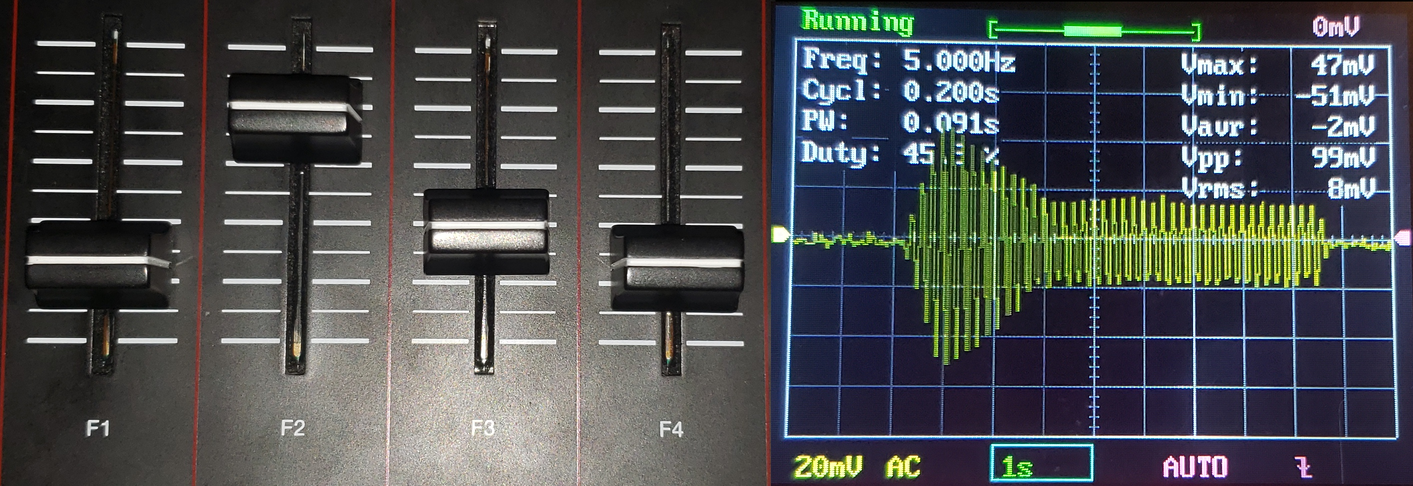
\includegraphics[width=\textwidth]{img/adsr2.png}
    \caption{ADSR 2}
    \label{fig:adsr2}
\end{figure}

\subsubsection{Mixer}

Given polyphony was to be implemented, there was a need for a module that could add all the operators together without overflow of data during addition, nor loss of amplitude. Since the human hand has 10 fingers, 12 operators were instantiated to cover all bases. The mixer was built to have 12 inputs and output a single signal. It does so by calculating how many extra bits are needed for the sum of all the signals. This can be done by taking a $\log_2$ of the number of signals added. Once this number is known, the signals are resized to the new size, added together, and then the upper bits are taken. The final signal is then multiplied by an amplitude value to allow for master volume control. The multiplication is done within a DSP slice on the FPGA to reduce the amount of logic and clock cycles needed to do the multiplication.

Figure \ref{fig:mixer} shows multiple signals being added together.

\begin{figure}[htb]
    \centering
    \begin{subfigure}{.49\textwidth}
        \centering
        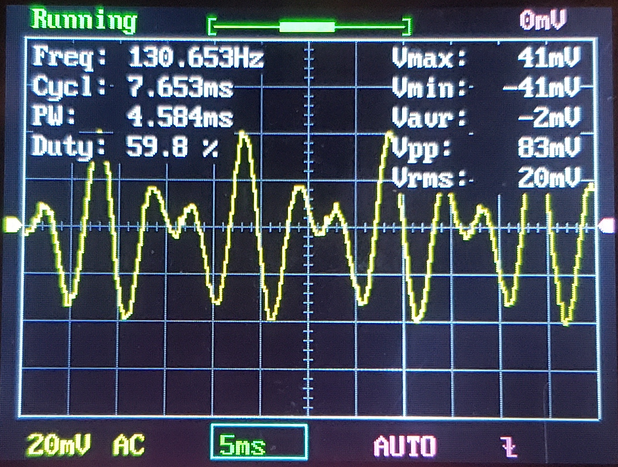
\includegraphics[width=0.96\linewidth]{img/sine_multi.png}
        \caption{Two sine waves}
        \label{fig:sine_multi}
    \end{subfigure}
    \begin{subfigure}{.49\textwidth}
        \centering
        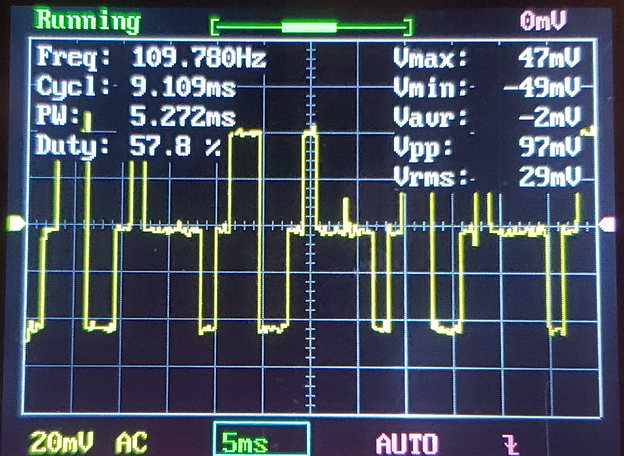
\includegraphics[width=\linewidth]{img/square_multi.png}
        \caption{Two square waves}
        \label{fig:square_multi}
    \end{subfigure}
    \caption{Signal addition in mixer module}
    \label{fig:mixer}
\end{figure}

\subsubsection{Audio Codec}

A large part of frustration in the assignment came from the audio codec. In truth, it presents a complex problem that is experienced in many modern hardware designs since it deals with the notion of multi-clock domains.

To start, the audio codec on the Nexys Video FPGA is the Analog Devices ADAU1761. It supports a wide variety of sample rates and up to 24bits of data per sample. It can be set up using I$^2$C, and audio data is sent over serial using I$^2$S. The original implementation used was one that was given for previous assignments; however, it had a number of issues, namely timing and setup. Because of this, the audio data was distorted, containing an audible compression and crunch within the sound on the output. Sample data was also sent one by one when needed as dictated by the clocks generated for I$^2$S communication. While the design worked for basic needs, because of the complexity of the synthesizer, these timing issues propagated through the design which created negative setup time issues during implementation, indicating possible loss of data. Indeed, when running the implemented design, no audio was being generated, even though sample data could be visible using console debug. This led to a re-implementation of the audio codec module.

The new design was actually based on an old one. Digilent had created a set of example projects to test out and learn the Nexys Video FPGA. The DMA project was used as reference and starting place for the changes necessary to fix the audio codec design. Initially, the only thing that was changed was the setup parameters as well as a flip flop cascade to sync the L/R clock with the system clock to know when the next sample was needed. This was implemented as a basic hardware project that had no high level complexity. With loopback testing and then testing with the Skarch Core, it was found that the new design produced a clean and loud audio signal that was no longer distorted. Given the codec seemed to be functioning as expected, the new design was put into placed and compiled. However, negative setup time was still being created and there was still no audio ouput when used in the MicroBlaze block design. This meant more research of the problem was needed.

A realization occurred that the system is partitioned into multiple clock domains. There was the system clock of 100 MHz and the audio codec clock which was 12.288 MHz. This meant that there would be syncing and phase issues between data, especially if the system was strained with complex designs. Research was done to find methods to mitigate cross-clock meta-stability issues and some methods were found such as two flip flop synchornizers, handshakes, and FIFOs \cite{edn_2014}. Upon investigating what the team at Digilent had done, it was seen that their design used an asynchronous FIFO system to mitigate the effects of the meta-stability since it would allow the two clock domains to transfer data at their own rates. These designs added quite a bit of complexity to the design, so they were initially avoided. First, duel flip flop synchronizers were tried to see if it would mitigate the problem. They brought the negative slack down, but did not fix the problem. Next, the clock generation for the audio codec was externalized since it's recommended to split the clock at one place instead of chaining clock dividers. This again lessened the problem, but did not fix it. Then, a set of FIFOs was implemented, but still, a considerable amount of negative slack remained. Finally, what had fixed the problem was adding in an asynchronous reset into the system since the reset provided by the AXI bus is synced to the 100 MHz system clock. Doing this allowed the bits that were clocked by the audio codec to meet timing requirements, and indeed, this fixed the issue.

\section{Running the Project}

Running the project is not exactly easy since it requires, aside from the FPGA, a MIDI circuit and MIDI controller. However, if all three components are available, then the project entails the following steps:

\begin{enumerate}
    \item Burn the Skrach Core bitstream onto the FPGA (this is due to a bug in the audio codec set up where first runs fails to generate audio output on the main project)
    \item Connect the MIDI circuit to pin 1 of the JC PMOD port
    \item Launch the SDK for the main project, if the sources aren't found, import them (Skrach and Skrach\_bsp under the Skrach.sdk folder)
    \item Compile, program FPGA with bitstream, and then run the program.
\end{enumerate}

In a console window of 115200 baud rate, you should receive a welcome message and then decode message from a MIDI controller if connected. Notes will automatically cause the Skrach Core to play signals on Line Out and Headphone jacks. Changing of signal type, master amplitude, and ADSR values are mapped to the controls on my keyboard which can correspond to different faders and knobs for different MIDI controllers. This can be remapped in the synth file. There were plans to allow for full control over USB UART, but that was not able to be implemented, so it's hard to test on the fly. However, debug prints can be uncommented and MIDI messages can be constructed statically within code to test the signal generator and code itself, as was done for easy testing early on.

\printbibliography[heading=bibintoc]
\end{document}
